\documentclass[conference]{IEEEtran}
\usepackage[utf8]{inputenc}
\usepackage{graphicx}
\usepackage[main=english,portuguese]{babel}

\usepackage{color,soul} % TEMPORARIO => SÓ PARA VISUALIZAR TEXTO PENDENTE

\ifCLASSINFOpdf
\else
\fi
\hyphenation{op-tical net-works semi-conduc-tor}


\begin{document}

\title{Sistema de visualização de\\redes metabólicas em grafo}

\author{\IEEEauthorblockN{Gabriella de O. Esteves}
\IEEEauthorblockA{Universidade de Brasília\\
Departamento de Ciência da Computação\\
Brasília, Brasil\\
Email: gabepk.ape@gmail.com}}


\maketitle

% As a general rule, do not put math, special symbols or citations
% in the abstract
\begin{abstract}
The abstract goes here.
\end{abstract}

% no keywords

\section{Introducão}

O metabolismo é isso X, ocorre por isso (síntese e degradação) e funciona com isso (moléculas, metabólitos).

Como o metabolismo tem sido representado computacionalmente (redes metabólicas)? Como as redes metabólicas tem sido visualizadas (estado da arte)? \\
Problema, objetivo. \\
Descrição dos capítulos.


\section{Redes Metabólicas}

\hl{FRASE INTRO} \indent AAAAAAA AAAAAAA  AAAAAAAA AAAAAAAAA AAAAAAAAAA AAAAA AAAAAAA AAAAAAA AAAAA AAAAAA AAAA AAAAA AAAAAAAA \\. As reações bioquímicas são alterações químicas que fornecem um ou mais produtos a partir de uma ou mais entradas, chamadas de substratos. Uma via metabólica é uma sequência de reações bioquímicas, cujo produto e subtrato são denominados de metabólitos, que podem ser catalisadas por enzimas, estas que muitas vezes necessitam de compostos químicos não-proteicos chamados de co-fatores para realizarem suas atividades na célula. O conjunto de vias metabólicas de um organismo é chamado de rede metabólica. Todos estes elementos que compõem as redes metabólicas são dados biológicos estudados na área metabolômica. Nesta seção serão apresentados três bancos de dados de redes metabólicas utilizadas em análise do metaboloma, KEGG, BIoCyc e Reactoma.

\subsection{Conceitos de Biologia Molecular}

O DNA é um conjunto de biomoléculas em um organismo que armazenam informações, chamados de genes, referentes ao funcionamento de todas as suas células. Ele constitui o genoma em todos os seres vivos, com excessão dos vírus. A expressão dos genes é o processo no qual os genes são filtrados e utilizados na síntese de um produto, geralmente proteína. O método é segmentado em três etapas: transcrição (síntese de RNA mensageiro, mRNA, a partir de DNA), \textit{splicing} (filtragem do gene síntetizador de proteínas desejadas do mRNA) e tradução (síntese de proteína a partir do mRNA filtrado). Completo este processo, as proteínas resultantes poderão formar uma configuração tridimensional de até quatro níveis. As enzimas, por exemplo, são proteínas que podem ter estrutura terciária ou quaternária. \\
\indent \hl{FALAR DE SEQUENCIAMENTO DE GENOMA} \indent AAAAAAA AAAAAAA  AAAAAAAA AAAAAAAAA AAAAAAAAAA AAAAA AAAAAAA AAAAAAA AAAAA AAAAAA AAAAA AAAAAA AAAA AAAAA AAAAAAAA AAAA AAAAA AAAAAAAA \\

\subsection{Conceitos de Metabolismo}

O papel das enzimas no metabolismo é realizar biosíntese/degradação de moléculas para produção de energia (catalisar) com o propósito de acelerar reações bioquímicas. Aquelas que possuem a mesma atividade enzimática porém estruturas físicas diferentes são chamadas isoenzimas. \hl{LIGAR PARAGRAFOS}. \indent AAAAAAA AAAAAAA  AAAAAAAA AAAAAAAAA AAAAAAAAAA AAAAA AAAAAAA \\
\indent Quando o metabolismo exerce uma função fundamental no organismo, ele é classificado como metabolismo primário. Mitose e meiose são exemplos de metabolismos primários. Já quando o metabolismo não está relacionado a reprodução, desenvolvimento ou crescimento, ele não é essencial no organismo e, portanto, secundário. Os metabólitos secundários, apesar da aparente insignificância, podem ser antibióticos, por exemplo, e deste modo são bastante aplicados na medicina e na indústria.

% CITAR MESTRADO DO WALDEYR

\subsection{Banco de Dados de redes metabólicas}


\hl{FRASE INTRO} \indent AAAAAAA AAAAAAA  AAAAAAAA AAAAAAAAA AAAAAAAAAA AAAAA AAAAAAA AAAAAAA AAAAA AAAAAA AAAAA AAAAAA AAAA AAAAA AAAAAAAA AAAA AAAAA AAAAAAAA \\. O KEGG (\textit{Kyoto Encyclopedia of Genes and Genomes}) é um repositório de ferramentas para análise de dados de sistemas biológicos em nível molecular, sobretudo para conjuntos de dados em larga escala gerados por sequenciamento de genoma. \hl{Citar:http://www.kegg.jp/kegg/kegg1a.html} O sistema é disponibilizado via \textit{web} pelo site \textit{http://www.genome.jp/kegg/}. As informações sobre os sistemas podem ser dadas em forma de módulo, unidades funcionais com identificação otimizada para análise dos dados, em forma de \textit{brite}, coleção de arquivos estruturados hierarquicamente sobre as funções das entidades biológicos, ou em forma de vias, mapa de interações moleculares e reações químicas. Dado que o metabolismo é um conjunto de reações e transformações químicas, a maneira natural de representá-lo é por meio de uma rede de interações, ou seja, em forma de vias. O KEGG oferece uma ferramenta de busca de vias metabólicas sobre várias rede metabólica, dos vários organismos que constituem o banco de dados. \hl{LIGAR PARAGRAFOS}.\\
\indent O BioCyc é um sistema de coleção de aproximadamente 7 mil bancos de dados chamados PGDBs (\textit{Pathway/Genome Databases}) pois possuem duas maneiras diferentes de representar as informações: modelo de vias metabólicas, que enfatiza as sequências de reações, substratos e produtos de múltiplos organismos, ou modelo de sequência genômica, que destaca a localização e descrição dos genes de cada organismo específico. \hl{Citar: http://biocyc.org/} . Os bancos PGDBs são organizado em três camadas de acordo com a frequência de atulizações/refinações e da maneira com que os dados foram obtidos. O BioCyc possui um banco de dados específico para redes metabólicas determinadas experimentalmente, chamado MetaCyc. \hl{LIGAR PARAGRAFOS}. AAAAAAA AAAAAAA  AAAAAAAA AAAAAAAAA AAAAAAAAAA AAAAA AAAAAAA AAAAAAA AAAAA AAAAAA AAAA AAAAA AAAAAAAA \\
\indent Reactoma é um banco de dados de reações de mudança de estado (não só reações bioquímica, mas também reações de ativação, de degradação e de ligação, por exemplo) \hl{Citar:http://wiki.reactome.org/index.php/Usersguide}. No sistema existe uma rede geral para cada organismo que representa os vários seus sistemas, como reprodução e metabolismo. Algumas subredes estão conectadas (por exemplo, replicação de DNA e ciclo de célula), outra não (por exemplo, contração muscular e reprodução). Nesta rede, cada nó representa uma via cujo número de entidade se reflete no raio do nó, e cada aresta representa a relação entre estas vias. O site ainda possui uma ferramenta de análise de dados baseada nas correspondências entre as reações na redes dos organismos comparados. \\
\hl{FRASE FINAL} \indent AAAAAAA AAAAAAA  AAAAAAAA AAAAAAAAA AAAAAAAAAA AAAAA AAAAAAA AAAAAAA AAAAA AAAAAA AAAA AAAAA AAAAAAAA \\

\section{Ferramentas de visualização de redes metabólicas}

\hl{PARAGRAFO INICIAL} AAAAAAA AAAAAAA  AAAAAAAA AAAAAAAAA AAAAAAAAAA AAAAA AAAAAAA AAAAAAA AAAAA AAAAAA AAAA AAAAA AAAAAAAA AAAAAAA AAAAAAA  AAAAAAAA AAAAAAAAA AAAAAAAAAA AAAAA AAAAAAA AAAAAAA AAAAA AAAAAA AAAA AAAAA AAAAAAAA 

\subsection{KEGG Pathway Maps}

O KEGG oferece uma visao geral e uma visualização específica para análise de redes metabólicas. Na primeira, o grafo interativo apresenta uma perspectiva global das entidades do banco de dados do KEGG, chamadas de objetos KEGG. Neste panorama, a rede metabólica selecionada é destacada e é acompanhada de interações externas, que não possuem ligação direta com a rede análisada. Os nós representam compostos químicos e as arestas podem representar enzimas, reações e/ou \hl{otholog}. Na página do Atlas, a visualização das arestas pode ser filtrada, bem como as vias, de acordo com suas funções. A Figura \ref{terpenoid_meva_kegg} apresenta uma parte da via de biosíntese de terpenóide, que tem início no composto Acetyl-CoA, destacada sobre as demais.

\begin{figure}[!t]
\centering
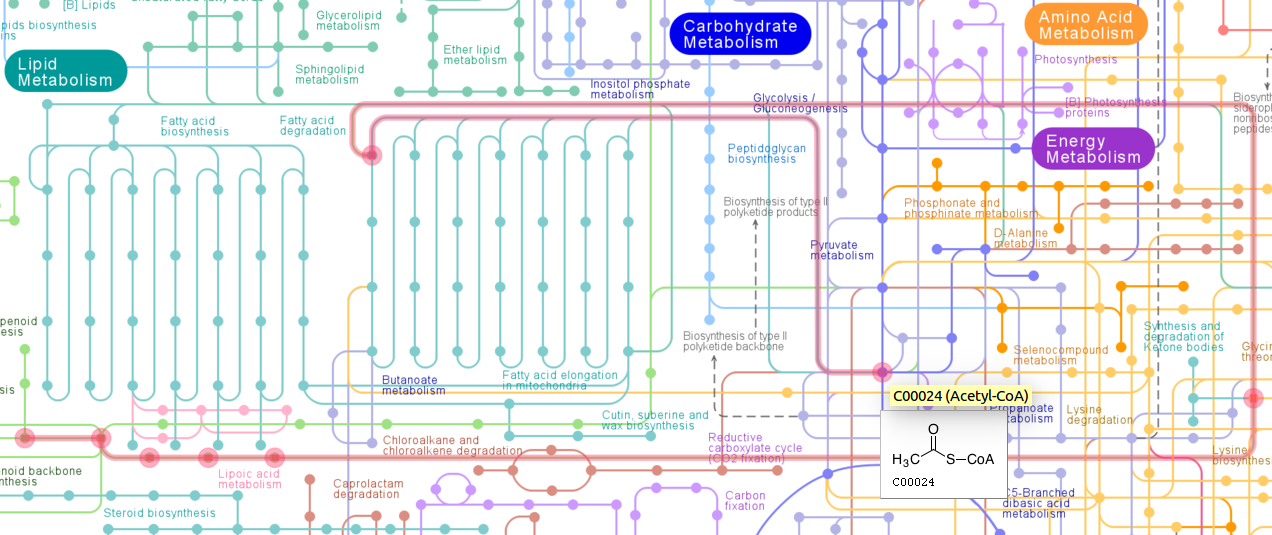
\includegraphics[width=0.5\textwidth]{terpenoid_meva_kegg.png}
\caption{KEGG}
\label{terpenoid_meva_kegg}
\end{figure}

Uma outra maneira de visualizar esta via é acessando o objeto KEGG do tipo map que ela representa (\textit{KEGG Pathway Map}). O mapa de vias é um diagrama de interações/reações moleculares desenhado manualmente. A via da Figura \ref{terpenoid_meva_kegg_solo} apresenta a mesma via da Figura \ref{terpenoid_meva_kegg}.

\begin{figure}[!t]
\centering
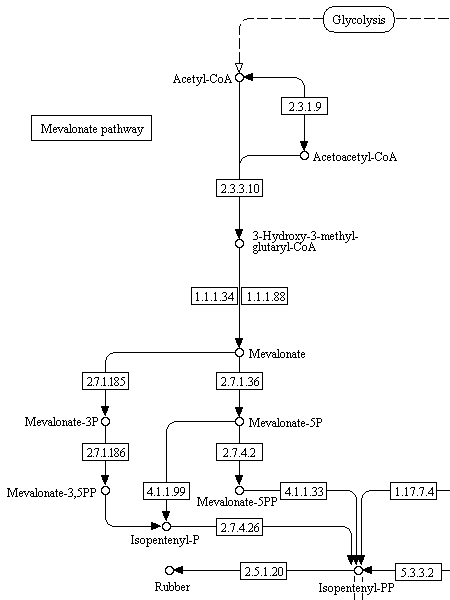
\includegraphics[width=0.35\textwidth]{terpenoid_meva_kegg_solo.png}
\caption{KEGG}
\label{terpenoid_meva_kegg_solo}
\end{figure}

\subsection{BioCyc}

\begin{figure}[!t]
\centering
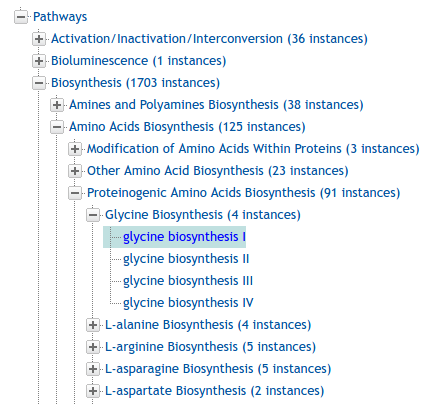
\includegraphics[width=0.5\textwidth]{metacyc_arvore.png}
\caption{BioCyc}
\label{metacyc_arvore}
\end{figure}


\begin{figure}[!t]
\centering
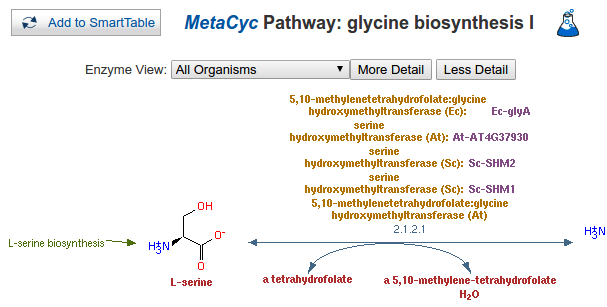
\includegraphics[width=0.5\textwidth]{metacyc_glycin_small.png}
\caption{BioCyc}
\label{metacyc_glycin_small}
\end{figure}


\subsection{Reactome}

\begin{figure}[!t]
\centering
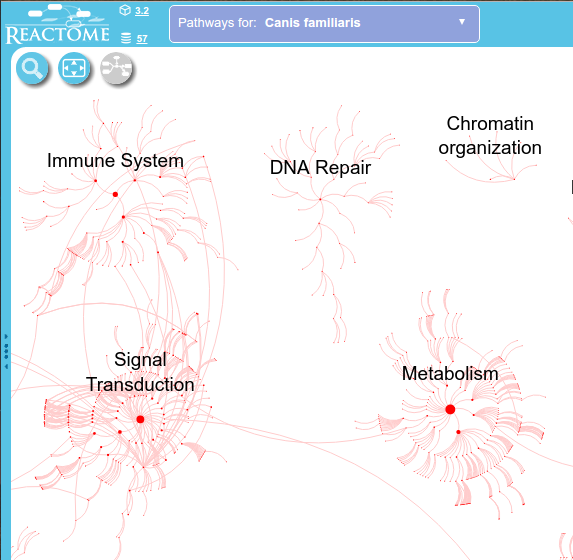
\includegraphics[width=0.5\textwidth]{reactome_canis_small.png}
\caption{Reactome}
\label{reactome_canis_small}
\end{figure}



\subsection{Cytoscape}





\section{Sistema 2Path}

\subsection{Banco de dados em grafo}

Waldeyr

\subsection{Sistema de consulta}

Gabriella

\section{Conclusão}

Conclusão





% An example of a floating figure using the graphicx package.
% Note that \label must occur AFTER (or within) \caption.
% For figures, \caption should occur after the \includegraphics.
% Note that IEEEtran v1.7 and later has special internal code that
% is designed to preserve the operation of \label within \caption
% even when the captionsoff option is in effect. However, because
% of issues like this, it may be the safest practice to put all your
% \label just after \caption rather than within \caption{}.
%
% Reminder: the "draftcls" or "draftclsnofoot", not "draft", class
% option should be used if it is desired that the figures are to be
% displayed while in draft mode.
%
%\begin{figure}[!t]
%\centering
%\includegraphics[width=2.5in]{myfigure}
% where an .eps filename suffix will be assumed under latex, 
% and a .pdf suffix will be assumed for pdflatex; or what has been declared
% via \DeclareGraphicsExtensions.
%\caption{Simulation results for the network.}
%\label{fig_sim}
%\end{figure}

% Note that the IEEE typically puts floats only at the top, even when this
% results in a large percentage of a column being occupied by floats.


% An example of a double column floating figure using two subfigures.
% (The subfig.sty package must be loaded for this to work.)
% The subfigure \label commands are set within each subfloat command,
% and the \label for the overall figure must come after \caption.
% \hfil is used as a separator to get equal spacing.
% Watch out that the combined width of all the subfigures on a 
% line do not exceed the text width or a line break will occur.
%
%\begin{figure*}[!t]
%\centering
%\subfloat[Case I]{\includegraphics[width=2.5in]{box}%
%\label{fig_first_case}}
%\hfil
%\subfloat[Case II]{\includegraphics[width=2.5in]{box}%
%\label{fig_second_case}}
%\caption{Simulation results for the network.}
%\label{fig_sim}
%\end{figure*}
%
% Note that often IEEE papers with subfigures do not employ subfigure
% captions (using the optional argument to \subfloat[]), but instead will
% reference/describe all of them (a), (b), etc., within the main caption.
% Be aware that for subfig.sty to generate the (a), (b), etc., subfigure
% labels, the optional argument to \subfloat must be present. If a
% subcaption is not desired, just leave its contents blank,
% e.g., \subfloat[].


% An example of a floating table. Note that, for IEEE style tables, the
% \caption command should come BEFORE the table and, given that table
% captions serve much like titles, are usually capitalized except for words
% such as a, an, and, as, at, but, by, for, in, nor, of, on, or, the, to
% and up, which are usually not capitalized unless they are the first or
% last word of the caption. Table text will default to \footnotesize as
% the IEEE normally uses this smaller font for tables.
% The \label must come after \caption as always.
%
%\begin{table}[!t]
%% increase table row spacing, adjust to taste
%\renewcommand{\arraystretch}{1.3}
% if using array.sty, it might be a good idea to tweak the value of
% \extrarowheight as needed to properly center the text within the cells
%\caption{An Example of a Table}
%\label{table_example}
%\centering
%% Some packages, such as MDW tools, offer better commands for making tables
%% than the plain LaTeX2e tabular which is used here.
%\begin{tabular}{|c||c|}
%\hline
%One & Two\\
%\hline
%Three & Four\\
%\hline
%\end{tabular}
%\end{table}


% Note that the IEEE does not put floats in the very first column
% - or typically anywhere on the first page for that matter. Also,
% in-text middle ("here") positioning is typically not used, but it
% is allowed and encouraged for Computer Society conferences (but
% not Computer Society journals). Most IEEE journals/conferences use
% top floats exclusively. 
% Note that, LaTeX2e, unlike IEEE journals/conferences, places
% footnotes above bottom floats. This can be corrected via the
% \fnbelowfloat command of the stfloats package.



% conference papers do not normally have an appendix


% use section* for acknowledgment
\section*{Agradecimento}


The authors would like to thank...





% trigger a \newpage just before the given reference
% number - used to balance the columns on the last page
% adjust value as needed - may need to be readjusted if
% the document is modified later
%\IEEEtriggeratref{8}
% The "triggered" command can be changed if desired:
%\IEEEtriggercmd{\enlargethispage{-5in}}

% references section
% manually copy in the resultant .bbl file
% set second argument of \begin to the number of references
% (used to reserve space for the reference number labels box)
\begin{thebibliography}{1}

\bibitem{IEEEhowto:kopka}
H.~Kopka and P.~W. Daly, \emph{A Guide to \LaTeX}, 3rd~ed.\hskip 1em plus
  0.5em minus 0.4em\relax Harlow, England: Addison-Wesley, 1999.

\end{thebibliography}





\end{document}


